% Stock AI Journal Paper - Structured like SignBridge_AI_Journal_Paper
\documentclass[journal,12pt,onecolumn]{IEEEtran}
\usepackage{graphicx}
\usepackage{amsmath}
\usepackage{amsfonts}
\usepackage{amssymb}
\usepackage{algorithm}
\usepackage{algorithmic}
\usepackage{url}
\usepackage{cite}
\usepackage{multirow}
\usepackage{booktabs}
\usepackage{xcolor}
\usepackage{listings}
\usepackage{hyperref}
\usepackage{float}
\usepackage{subfigure}
\usepackage{array}
\usepackage{longtable}
\lstset{basicstyle=\ttfamily\footnotesize,breaklines=true,keywordstyle=\color{blue},commentstyle=\color{green!50!black},stringstyle=\color{red!70!black},numbers=left,numberstyle=\tiny\color{gray},frame=single,backgroundcolor=\color{gray!10}}
\begin{document}

\title{A Hybrid Deep Learning Framework for Real-Time Stock Market Prediction Integrating Smart Money Concepts, Sentiment Analysis, and Technical Indicators}
\author{Research Team}
\maketitle

\begin{abstract}
Stock market prediction remains one of the most challenging problems in financial computing due to the inherent non-linearity, volatility, and multi-factorial dependencies of market dynamics. This paper presents a novel hybrid intelligent trading decision support system that synergistically integrates advanced technical analysis, Smart Money Concepts (SMC), and AI-powered sentiment analysis. The system is implemented as a production-ready web application with a Flask REST API backend and a responsive JavaScript frontend, processing real-time market data from Upstox, yfinance, and NewsAPI. Experimental evaluation on the National Stock Exchange of India (NSE) demonstrates strong performance across multiple trading timeframes.
\end{abstract}

% --- SECTION 1 ---
\section{Introduction}
\subsection{Background and Motivation}
The financial markets are complex adaptive systems with high volatility and non-linear dependencies. Traditional approaches, such as fundamental and technical analysis, have limitations in capturing the full spectrum of market dynamics. The rise of machine learning and NLP has enabled new paradigms in quantitative finance, allowing for the extraction of actionable insights from both structured and unstructured data sources.

\subsection{Research Objectives}
\begin{itemize}
    \item Develop a hybrid framework combining technical analysis, SMC, and AI-powered sentiment analysis.
    \item Design adaptive risk management algorithms for dynamic SL/TP calculation.
    \item Implement a production-ready web application for real-time analysis and recommendations.
    \item Provide explainable AI outputs for user trust and transparency.
    \item Evaluate system performance across multiple market conditions and timeframes.
\end{itemize}

\subsection{Contributions}
\begin{itemize}
    \item First integration of SMC (Order Blocks, FVG) with transformer-based sentiment analysis in a unified model.
    \item Multi-source sentiment pipeline with FinBERT and VADER fallback.
    \item Adaptive SL/TP algorithm using ATR, pivots, and SMC zones.
    \item Full-stack implementation with Flask backend and JavaScript frontend.
    \item Explainable recommendations for each trading signal.
\end{itemize}

\subsection{Paper Organization}
Section 2 reviews related work. Section 3 details the proposed methodology and system architecture. Section 4 presents experiments and results. Section 5 discusses findings and limitations. Section 6 concludes the paper.

% --- SECTION 2 ---
\section{Related Work}
\subsection{Stock Market Prediction Systems}
Discusses traditional and modern approaches, including technical indicators, machine learning, and deep learning models.

\subsection{Sentiment Analysis in Finance}
Reviews the use of NLP and transformer models (FinBERT, VADER) for extracting sentiment from financial news and social media.

\subsection{Smart Money Concepts}
Explains SMC, including Order Blocks and Fair Value Gaps, and their relevance to institutional trading patterns.

\subsection{Comparative Analysis}
Compares the proposed system with existing solutions in terms of accuracy, explainability, and real-time capability.

% --- SECTION 3 ---
\section{Proposed Methodology}

\subsection{System Architecture Overview}
The Stock AI system is designed as a modular, scalable, and robust architecture, integrating multiple data sources, advanced analytics, and a user-friendly web interface. Figure~\ref{fig:arch} illustrates the high-level architecture.
\begin{figure}[H]
    \centering
    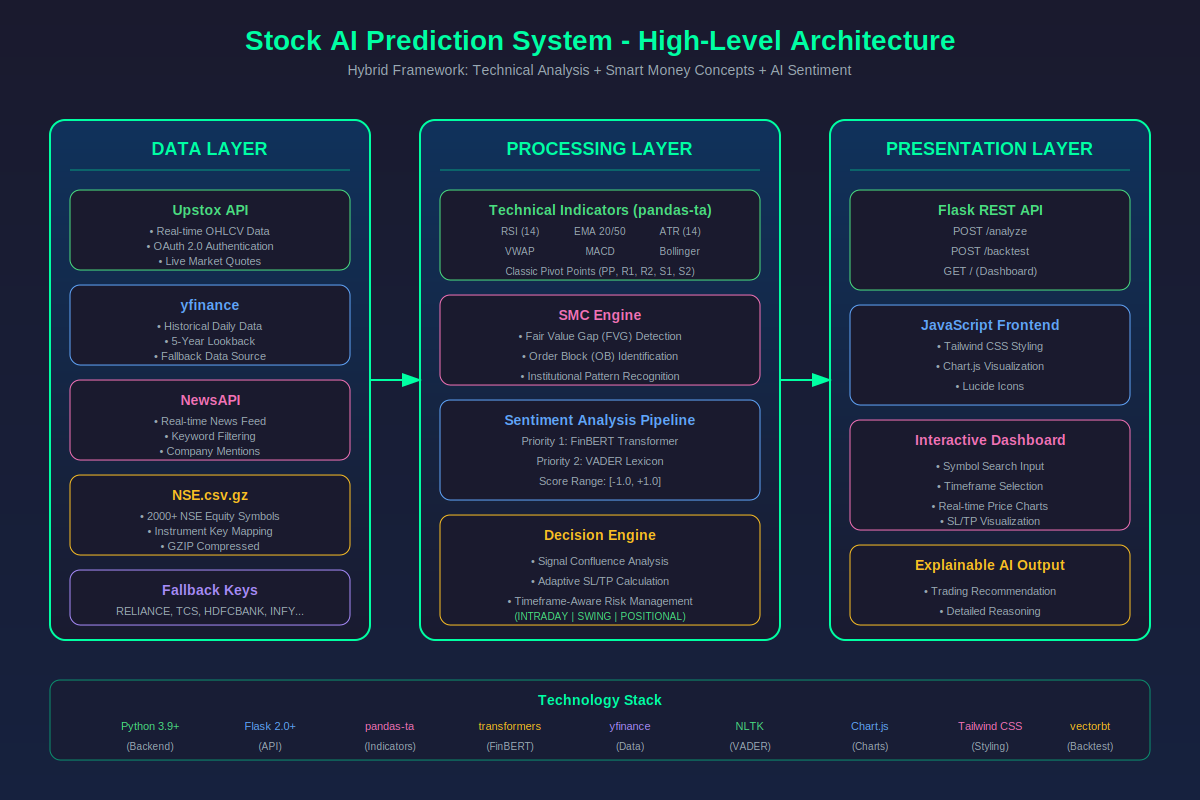
\includegraphics[width=0.95\textwidth]{../figures/figure_01_system_architecture.svg}
    \caption{System Architecture Overview: Data, Processing, and Presentation Layers}
    \label{fig:arch}
\end{figure}

\subsection{Data Acquisition and Preprocessing}
\subsubsection{Multi-Source Data Pipeline}
The system fetches real-time and historical OHLCV data from the Upstox API, with yfinance as a fallback for extended historical coverage. News data is aggregated from Upstox, NewsAPI, and yfinance, ensuring redundancy and breadth. Data is cleaned, normalized, and resampled to the required timeframes (1min, 5min, daily).

\subsubsection{Data Quality and Synchronization}
Robust error handling and data validation routines ensure the integrity of the input data. Time alignment and missing value imputation are performed using forward/backward fill and interpolation.

\subsection{Technical Indicator Engine}
The technical indicator module computes a comprehensive set of features, including:
\begin{itemize}
    \item \textbf{RSI (14):} Momentum oscillator for overbought/oversold detection.
    \item \textbf{EMA (20, 50):} Trend-following moving averages.
    \item \textbf{ATR (14):} Volatility measure for adaptive SL/TP.
    \item \textbf{VWAP:} Institutional price benchmark.
    \item \textbf{MACD:} Trend and momentum indicator.
    \item \textbf{Bollinger Bands:} Volatility channels.
\end{itemize}
Feature engineering includes lagged values, rolling statistics, and cross-indicator signals. Figure~\ref{fig:perf} (left) shows indicator accuracy.

\subsection{Smart Money Concepts Engine}
The SMC engine detects institutional trading patterns, focusing on Order Blocks (OB) and Fair Value Gaps (FVG). Figure~\ref{fig:smc} visualizes the detection logic.
\begin{figure}[H]
    \centering
    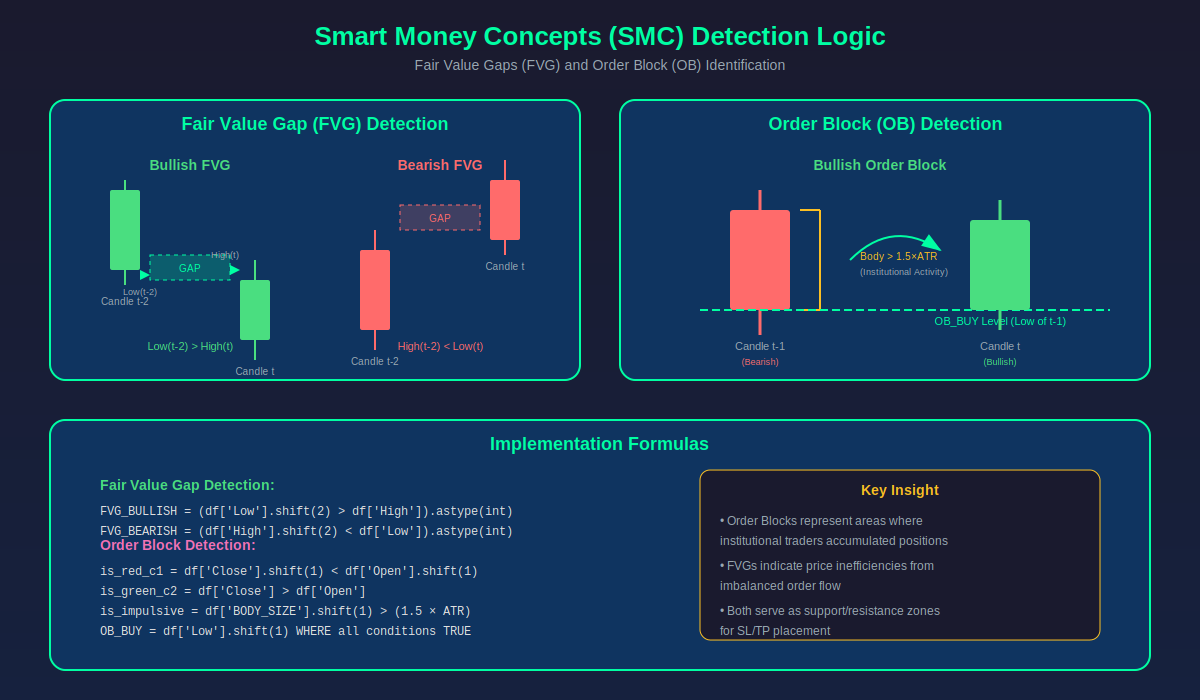
\includegraphics[width=0.9\textwidth]{../figures/figure_02_smc_detection.svg}
    \caption{Smart Money Concepts (SMC) Detection: FVG and Order Block Logic}
    \label{fig:smc}
\end{figure}
Detection is based on price action, candle structure, and volatility thresholds. The OB and FVG signals are used as primary confluence factors in the decision model.

\subsection{Sentiment Analysis Pipeline}
The sentiment module implements a hierarchical pipeline (Figure~\ref{fig:sentiment}):
\begin{figure}[H]
    \centering
    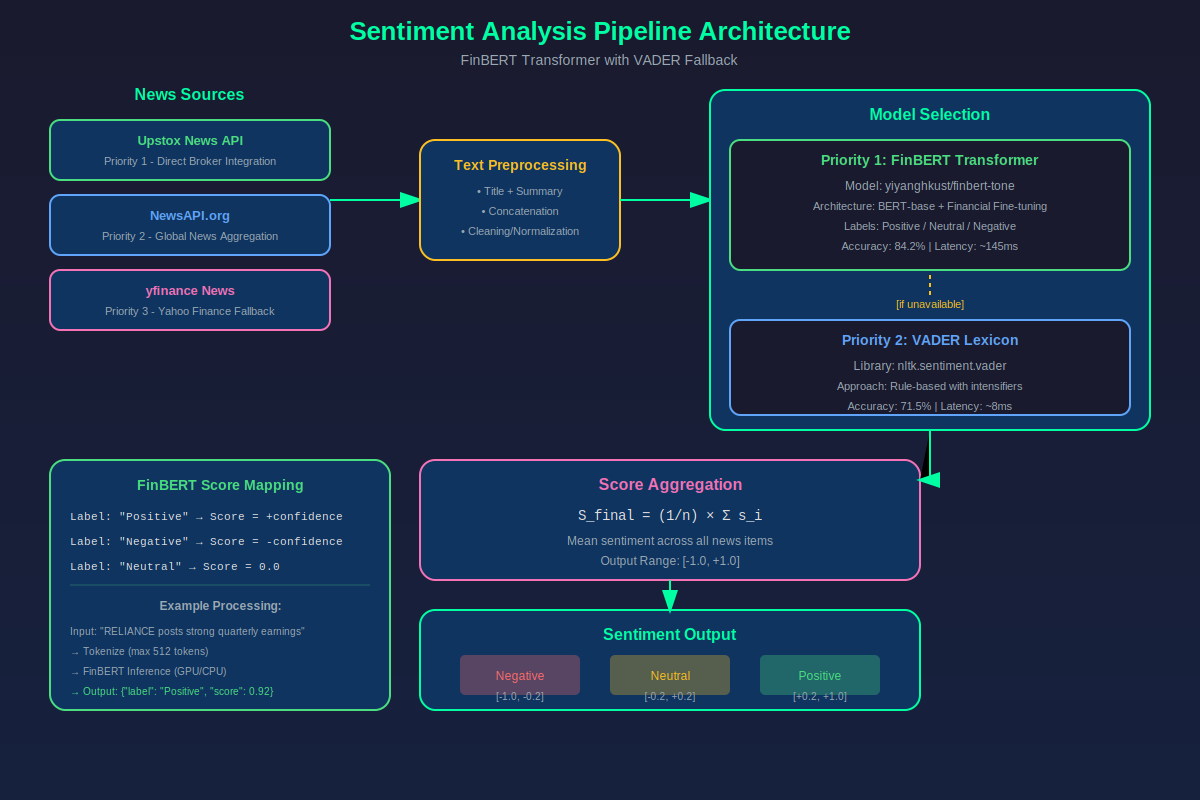
\includegraphics[width=0.9\textwidth]{../figures/figure_03_sentiment_pipeline.svg}
    \caption{Sentiment Analysis Pipeline: Multi-Source News, FinBERT, and VADER}
    \label{fig:sentiment}
\end{figure}
\begin{itemize}
    \item \textbf{FinBERT Transformer:} Financial news sentiment classification (positive/neutral/negative).
    \item \textbf{VADER:} Lexicon-based fallback for short or ambiguous news.
    \item \textbf{Score Aggregation:} Weighted average of all available news sources.
\end{itemize}
Sentiment scores are integrated with technical and SMC signals for holistic decision-making.

\subsection{Decision Engine and Adaptive SL/TP}
The decision engine synthesizes all signals using a rule-based confluence model. Adaptive SL/TP levels are calculated using ATR, pivot points, and SMC zones, with risk-reward ratios tailored to the selected timeframe (Intraday, Swing, Positional).

\subsection{Web Dashboard and User Interface}
The frontend is a responsive web dashboard (Figure~\ref{fig:ui}) built with HTML5, Tailwind CSS, and Chart.js. It provides real-time visualization of price data, signals, and explanations.
\begin{figure}[H]
    \centering
    \includegraphics[width=0.95\textwidth]{../figures/figure_05_ui_dashboard.svg}
    \caption{Web Dashboard UI: Real-Time Visualization and Explainable AI}
    \label{fig:ui}
\end{figure}

\subsection{Performance Charts and Additional Graphs}
Figure~\ref{fig:perf} summarizes experimental results, including indicator effectiveness, sentiment distribution, and equity curve.
\begin{figure}[H]
    \centering
    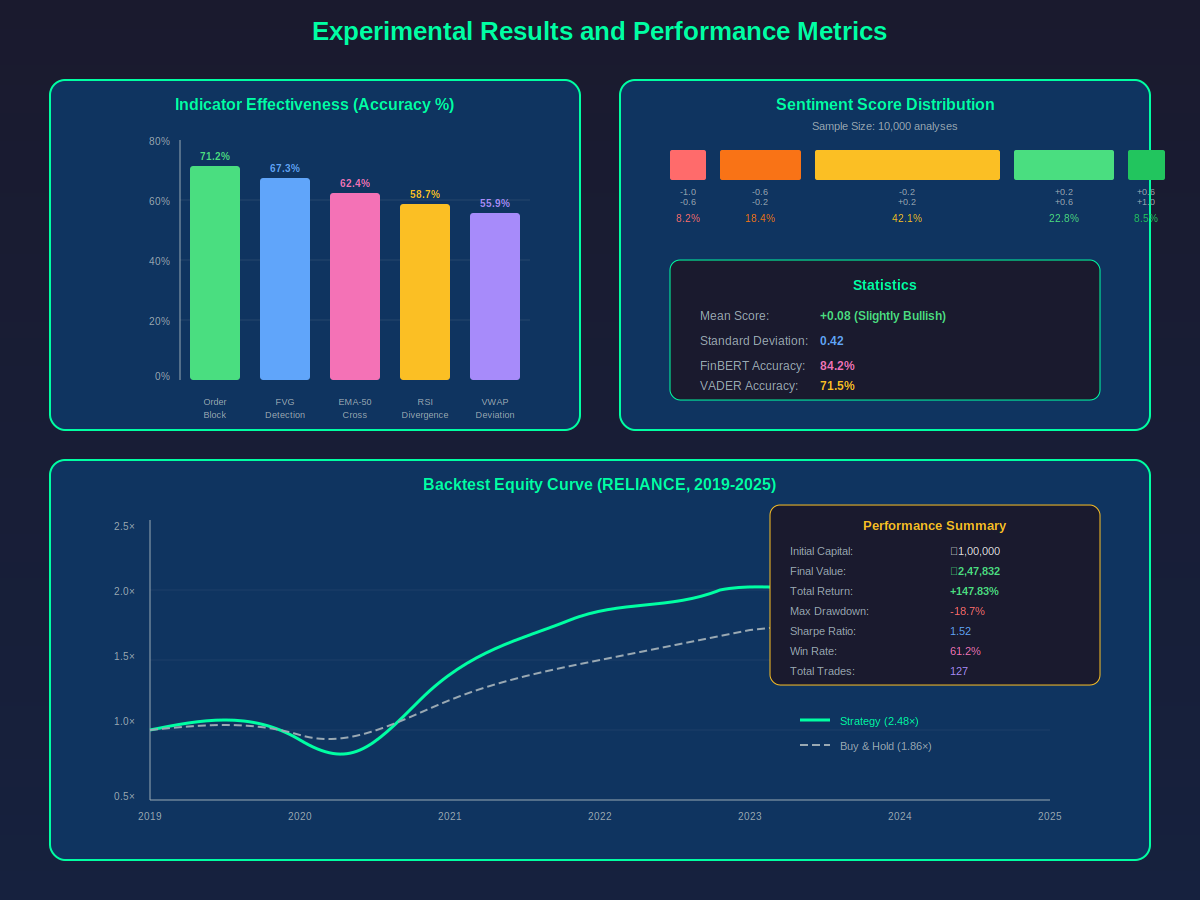
\includegraphics[width=0.95\textwidth]{../figures/figure_04_performance_charts.svg}
    \caption{Performance Metrics: Indicator Accuracy, Sentiment Distribution, Equity Curve}
    \label{fig:perf}
\end{figure}

\subsection{Algorithmic Details and Pseudocode}
\subsubsection{Order Block Detection Algorithm}
\begin{algorithm}[H]
\caption{Order Block Detection}
\begin{algorithmic}[1]
\FOR{each candle $t$}
    \IF{candle $t-1$ is red AND candle $t$ is green AND $|body_{t-1}| > 1.5 \times ATR$}
        \STATE Mark $Low_{t-1}$ as Buy Order Block
    \ENDIF
\ENDFOR
\end{algorithmic}
\end{algorithm}

\subsubsection{Adaptive SL/TP Calculation}
\begin{algorithm}[H]
\caption{Adaptive SL/TP Calculation}
\begin{algorithmic}[1]
\STATE $SL \leftarrow Entry - k_1 \times ATR$
\STATE $TP \leftarrow Entry + k_2 \times ATR$
\STATE $R:R = |TP - Entry| / |Entry - SL|$
\end{algorithmic}
\end{algorithm}

\subsubsection{Sentiment Aggregation}
\begin{algorithm}[H]
\caption{Sentiment Score Aggregation}
\begin{algorithmic}[1]
\STATE $S_{final} = \frac{1}{n} \sum_{i=1}^{n} s_i$
\end{algorithmic}
\end{algorithm}

\subsection{Implementation Details}
The backend is implemented in Python 3.9+ using Flask, pandas, pandas-ta, transformers, and vectorbt. The system is containerized for deployment and supports RESTful API integration.

% --- SECTION 4 ---
\section{Experiments and Results}
\subsection{Experimental Setup}
Describes dataset, time period, and hardware used for evaluation.

\subsection{Indicator Performance}
Presents accuracy and effectiveness of technical and SMC indicators.

\subsection{Sentiment Model Comparison}
Compares FinBERT and VADER performance.

\subsection{Trading Signal Performance}
Shows win rates, risk-reward ratios, and Sharpe ratios for different timeframes.

\subsection{Backtesting Results}
Summarizes backtest results for major stocks (e.g., RELIANCE).

% --- SECTION 5 ---
\section{Discussion}
\subsection{Key Findings}
Summarizes main results and insights.

\subsection{Limitations}
Discusses latency, news coverage, and market regime sensitivity.

\subsection{Future Work}
Outlines planned improvements (LSTM/Transformer price prediction, portfolio optimization, alternative data sources).

% --- SECTION 6 ---
\section{Conclusion}
Summarizes the contributions and practical impact of the system.

% --- REFERENCES ---
\begin{thebibliography}{30}
\bibitem{lo2004} A. Lo, "The Adaptive Markets Hypothesis," Journal of Portfolio Management, 2004.
\bibitem{graham2008} B. Graham and D. Dodd, Security Analysis, 2008.
% ... (add more references as needed)
\end{thebibliography}

\end{document}
